\documentclass[12pt,a4paper]{report}
\usepackage[english]{babel}
\usepackage[utf8]{inputenc}
\usepackage{color}
\usepackage{amsmath}
\usepackage{mathtools}
\usepackage{graphicx}
\usepackage[export]{adjustbox}
\usepackage{subcaption} 
\usepackage{array}
\usepackage{multirow}
\usepackage{tabularborder}
\usepackage{footnote}
\usepackage{caption}
\usepackage{siunitx}
\usepackage{newlfont}
\usepackage{color}
\usepackage{url}
\def\UrlBreaks{\do\/\do-}
\usepackage{breakurl}
\usepackage{hyperref}
\usepackage{enumitem}
\textwidth=450pt\oddsidemargin=0pt
\usepackage{fancyhdr}
\pagestyle{fancy}
\usepackage[Lenny]{fncychap}
\usepackage{standalone}
\setlength{\headheight}{15pt}

\usepackage[backend=biber,style=numeric,autocite=plain,sorting=none]{biblatex}
\usepackage{csquotes} % When using babel or polyglossia with biblatex
\addbibresource{bibliography.bib}


\begin{document}
\begin{titlepage}
    %
    %
    % ONCE YOU ARE FINISHED WITH YOUR CHANGES MODIFY "RED" WITH "BLACK" IN ALL \textcolor COMMENTS
    %
    %
    \begin{center}
    {{\Large{\textsc{Alma Mater Studiorum $\cdot$ University of  Bologna}}}} 
    \rule[0.1cm]{15.8cm}{0.1mm}
    \rule[0.5cm]{15.8cm}{0.6mm}
    \\\vspace{3mm}
    {\small{\bf School of Science \\
    Department of Physics and Astronomy\\
    Master Degree in Physics}}
    \end{center}
    
    \vspace{23mm}
    
    \begin{center}\textcolor{black}{
    %
    % INSERT THE TITLE OF YOUR THESIS
    %
    {\Large{\bf Implementation of an automated pipeline for predicting the response to neo-adjuvant chemo-rediotherapy of colorectal cancer}}
    }\end{center}
    
    \vspace{50mm} \par \noindent
    
    \begin{minipage}[t]{0.47\textwidth}
    %
    % INSERT THE NAME OF THE SUPERVISOR WITH ITS TITLE (DR. OR PROF.)
    %
    {\large{\bf Supervisor: \vspace{2mm}\\\textcolor{black}{
    Prof. Gastone Castellani}\\\\
    %
    % INSERT THE NAME OF THE CO-SUPERVISOR WITH ITS TITLE (DR. OR PROF.)
    %
    % IF THERE ARE NO CO-SUPERVISORS REMOVE THE FOLLOWING 5 LINES
    %
    \textcolor{black}{
    \bf Co-supervisor: \vspace{2mm}\\Dr. Nico Curti\\\\}}}
    \end{minipage}
    %
    \hfill
    %
    \begin{minipage}[t]{0.47\textwidth}\raggedleft \textcolor{black}{
    {\large{\bf Submitted by:
    \vspace{2mm}\\
    %
    % INSERT THE NAME OF THE GRADUAND
    %
    \textcolor{black}{
    Giuseppe Filitto}}}
    }
    \end{minipage}
    
    \vspace{32mm}
    
    \begin{center}
    %
    % INSERT THE ACADEMIC YEAR
    %
    Academic Year \textcolor{black}{ 2020/2021}
    \end{center}
    
    \end{titlepage}

\documentclass{standalone}



\begin{document}

\begin{abstract}
Colorectal cancer is a malignant neoplasm of the large intestine resulting from the uncontrolled proliferation of one of the cells making up the colorectal tract. 
\\
In order to get information about diagnosis, therapy evaluation on colorectal cancer, analysis on radiological images can be performed through the application of dedicated algorithms.
Up to now, this process is performed using manual or semi-automatic techniques, which are time-consuming and highly operator dependent.
\\
The aim of this project is to develop and apply an automated pipeline to predict the response to neoadjuvant chemo-radiotherapy of patients affected by colorectal cancer.
Here, we propose an approach based on automatic segmentation and radiomic features extraction.
The segmentation process exploits a Convolutional Neural Network like U-Net, trained with medical annotations to perform the segmentation of the tumor areas.
Then, from the segmented regions, radiomic features are extracted and analyzed to obtain the prediction of response, based on the Tumor Regression Grade (TRG).
\\
We tested and developed our pipeline on MRI scans provided by the IRCCS Sant’Orsola-Malpighi Polyclinic.
The performance of the pipeline was measured for the segmentation purpose and for the prediction of response.
The results of these preliminary tests show that the pipeline is able to achieve a segmentation consistent with the medical annotations and a Dice Similarity Coefficient (DSC) coherent with literature.
Even for the prediction of response, the results show that the pipeline is able to correctly classify most of the cases.


\end{abstract}

\end{document}

\clearpage

\thispagestyle{empty}
\begin{flushright}
\null\vspace{\stretch{1}}
\large{\emph{\dots To my family and Nicole}}
\vspace{\stretch{2}}\null
\end{flushright}

\clearpage

\tableofcontents

\documentclass{standalone}

\begin{document}
\chapter*{Introduction}\addcontentsline{toc}{chapter}{Introduction}
\markboth{INTRODUCTION}{}

Colorectal cancer is a malignant neoplasm of the large intestine resulting from the uncontrolled proliferation of the cells making up the colorectal tract.
Colorectal cancer is the second malignant tumor per number of deaths after the lung cancer and the third for number of new cases after the breast and lung cancer\cite{cancerstats}.\\
Among the risk factors for this kind of cancer, non hereditary could range from colon polyps to long-standing ulcerative colitis, from Crohn's disease to old age. 
Also genetic history (HNPCC or Lynch syndrome) and nutritional factors as diabetes II can increase the probability of develop cancer \cite{tesicoppola}.
Preventive measures for colorectal cancer include physical activity, reducing the consumption of processed meat and alcohol, and avoiding smoking\cite{stats2019}.
\begin{figure}[h!]
	\centering
	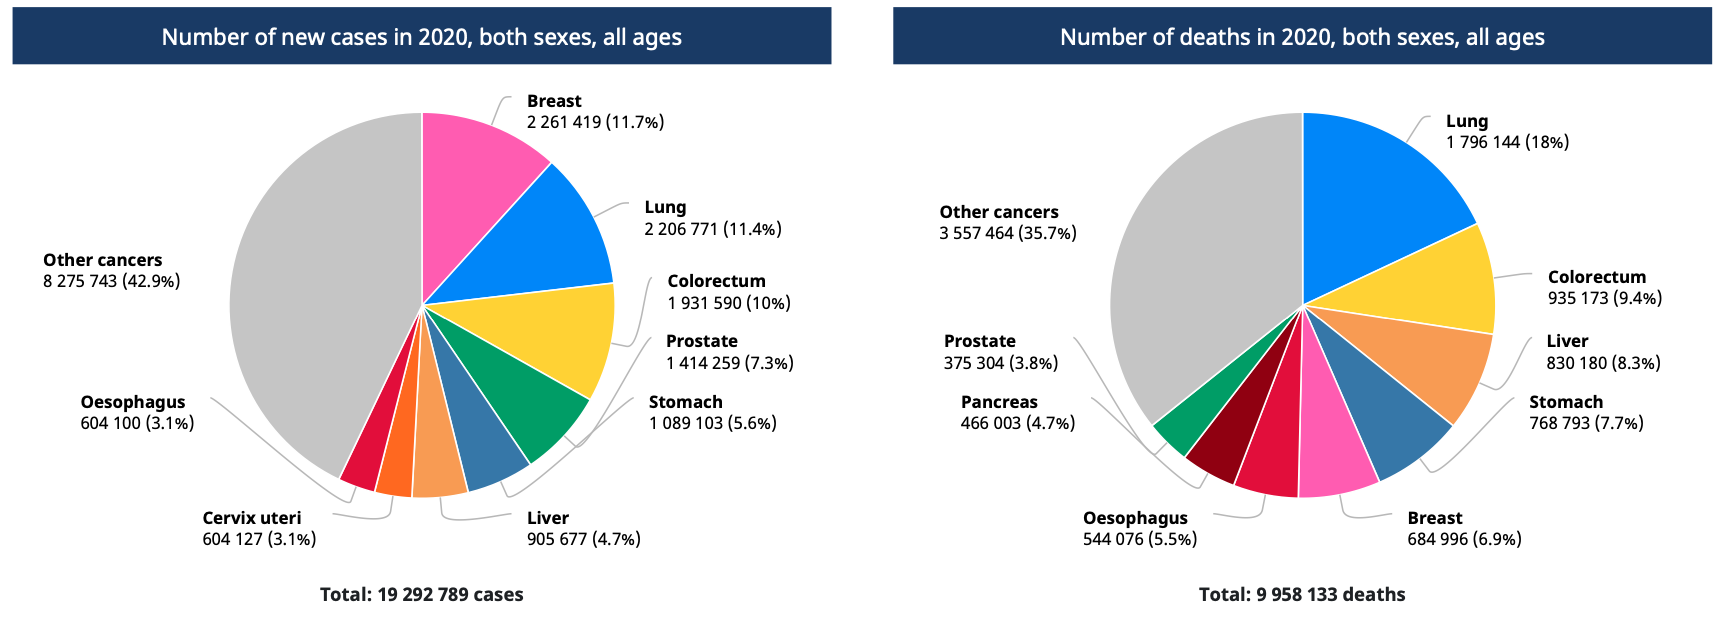
\includegraphics[width=\linewidth]{../images/cancerstats.png}
	\caption{World's cancer cases and deaths. From \cite{cancerstats} }
\end{figure}
\\
Screening and diagnosis methods for colorectal cancer can be based on different techniques. 
The gold standard in medical routines is colonoscopy which is an invasive technique\cite{jovana}.
Among medical imaging techniques, Magnetic Resonance Imaging (MRI) and Computed Tomography (CT) are the most used\cite{tesicoppola}. 
In particular Magnetic Resonance Imaging (MRI) is used for pre-operative predictions and for the evaluation of the neo-adjuvant therapy of patients affected by colorectal cancer \cite{tesicoppola}.

\begin{figure}[htp]

    \centering
    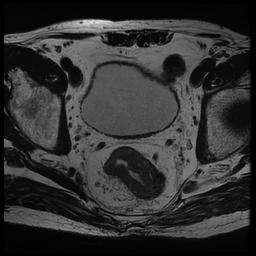
\includegraphics[width=.3\textwidth]{../images/T2AX_Alta_8.png}\hfill
    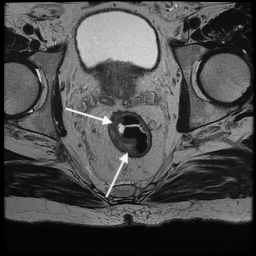
\includegraphics[width=.3\textwidth]{../images/T2AX_BO11_5.png}\hfill
    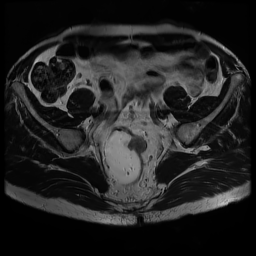
\includegraphics[width=.3\textwidth]{../images/T2AX_BO1_9.png}
    
    \caption{Example of MRI scans of patients affected by colorectal cancer. From Sant'Orsola original Dataset.}
    \label{trittico}
    
    \end{figure}
In order to get information about diagnosis, therapy evaluation, stage of colorectal cancer, analysis on radiological images can be performed through the application of dedicated algorithms.\\
In this scenario, the correct and fast identification of the cancer regions is a fundamental task. 
Up to now, this segmentation task is performed using manual or semi-automatic techniques, which are time-consuming (requiring hours per day) and subjected to the operator expertise since it requires the interaction with trained specialists\cite{tesicoppola, jovana}.
Moreover, due to the highly sensitivity to the operator expertise, the  obtained results cannot be reproduced\cite{Trebeschi2017}.
To overcome these issues, an automatic and fast way is required.\\
The aim of this project is to provide an automated pipeline to predict the response to neo-adjuvant chemo-radiotherapy of patients affect by colorectal cancer. 
The work is based and tested on MRI scans provided by IRCCS Sant’Orsola-Malpighi Policlinic.\\
The discussion will start focusing on medical digital images to understand their properties and features.
After that, an overview on the main segmentation method for the identification of the cancer regions will be given.
Then, the main pipeline characteristics and structure will be described.
In particular, how the segmentation was achieved using a Convolutional Neural Network and how extracting and processing medical image features.
Finally, the result will be shown and discussed.





\end{document}
\documentclass{standalone}
\begin{document}

    % MATERIALS AND METHODS
    \documentclass{standalone}
\begin{document}
\chapter{Results}
This Chapter will be aimed to show and discuss the results of the developed pipeline.
First of all, a brief description of the Dataset provided by the IRCCS Sant’Orsola-Malpighi Policlinic will be provided.
Then, the accuracy of the segmentation and of the prediction of response.
Finally, the outputs of the implementation will be shown.

\end{document}

    % MEDICAL DIGITAL IMAGES
    \documentclass{standalone}
\begin{document}
\section{Medical Digital Images}

A medical digital image is the digital representation of the anatomical (or functional) structure of the patient.
It is composed by a finite number of elements called \textit{pixels}.
A pixel is a discrete numeric representation of intensity or gray-level. It is an output coming from a two-dimensional function $f(x, y)$. 
The input of this function consists in the spatial coordinates, denoted with $(x, y)$ on the x-axis and y-axis of the image plane\cite{Gonzalez}.\\
A digital image can be processed by computers.
This process is called \textit{digital image processing} and it can be divided into two main categories: (\textit{image processing}) and (\textit{image analysis}).
The former includes methods whose output and input data are images.
The latter includes methods whose input data can be images and the output data are attributes extracted from the images.
\end{document}


        % GENERAL PROPERTIES 
        \documentclass{standalone}
\begin{document}
\subsection{General Properties}
The physical meaning of the image data depends on the performed image modality.
For example, Computed Tomography (CT) and Magnetic Resonance Imaging (MRI), give structural information about the anatomy of the patient.
Other techniques, such as Positron Emission Tomography (PET) or Functional Magnetic Resonance Imaging (fMRI) give information about the functional properties of the patient's target organs. 
However, we can distinguish some general characteristics of digital images:

\paragraph{Pixel depth} is the number of bits used to encode the values of each pixel and it is related to the memory space used to store the amount of the encoded information\cite{Larobina}. 
Higher the number of bits, higher the information stored but more memory space is required\cite{Larobina}. 
A group of 8 bits is called \textit{byte} and represent the smallest quantity that can be stored in the memory of a computer.
For example, if an image has a pixel depth of 16 or 12 bits the computer will always store two bytes per pixel\cite{Larobina}.
With a pixel depth of 8 bits it is possible to codify and store integer numbers between 0 and 255 $(2^8-1)$.
There are also two formats for the encoding in binary of floating-point numbers: single precision 32-bit and double precision 64-bit.

\paragraph{Pixel data} represent numerical values of the pixels stored according to the data type.
Pixel data can be complex values even if this data type is not common and can be bypassed by storing the real and imaginary parts as separate images.
For example, complex data are provided in MRI acquired data before the reconstruction (the so called k-space)\cite{Larobina}.


\paragraph{Metadata} are information that describe the image. It is usually stored at the beginning of the file as a header\cite{Larobina}. 
In the case of medical images, metadata have an important role due to the nature of the images.
For example, a magnetic resonance image might have parameters related to the pulse sequence used, timing information, number of acquisitions while a PET image might have information about the radiopharmaceutical injected and the weight of the patient.


\end{document}

        % MEDICAL IMAGE FORMATS
        \documentclass{standalone}
\begin{document}
    
\subsubsection{DICOM Format}

Image file formats provide a standard way to store information of an image in a computer file\cite{biondi}.
DICOM is the acronym of Digital Imaging and COmmunications in medicine.
It is not only a file format but also a network communication protocol\cite{Larobina}.
However here, we will discuss DICOM only as a medical image format.\\
DICOM file format establishes that the pixel data cannot be separated from the metadata\cite{Larobina}.
In other words, metadata and pixel data are merged in a unique file.
The header contains the description of the entire procedure used to generate the image in terms of acquisition protocol and scanning parameters\cite{Larobina}. 
It also contains patient information such as name, gender, age. 
For these reasons, the DICOM header is modality-dependent and varies in size. 
In practice, the header allows the image to be \textit{self-descriptive}.

\end{document}

        % SPATIAL DOMAIN FILTERING
        \documentclass{standalone}
\begin{document}
\section{Spatial Domain Filtering}


Filtering is a procedure used for modifying or enhancing an image.
The value of any given pixel in the output image is determined by applying some operations to the neighborhood of the corresponding input pixel.
A pixel's neighborhood is some set of pixels, defined by their locations relative to that pixel.
The term \textit{spatial domain} indicates that the procedures operate directly on pixels.
Mathematically:

\begin{equation}
    g(x,y) = T[f(x,y)] 
\end{equation}

where $f(x, y)$ is the input image, $g(x, y)$ the output image and $T$ is an operator on $f$ defined over some neighborhood of $(x, y)$.
The operation on the point located in $(x, y)$ usually involves the application of a matrix called \textit{mask} or \textit{kernel}.
The application of the above-mentioned mask (or kernel) on an image is called \textit{spatial filtering}.
Filtering creates a new pixel with the same coordinates of the center of the neighborhood, whose value is the result of the operation.
For each $(x, y)$ of the image, the filter transform $g(x, y)$ is the linear combination of the mask coefficient $w(s, t)$ and the pixels of the image affected by the mask itself.
In general, we can write:
\begin{equation}
    g(x, y) = \sum_{s = -a}^{a} \sum_{t = -b}^{b} w(s, t) f(x + s, y + t)
\end{equation}  

\begin{figure}[ht]

    \centering
    \includegraphics[width=.9\textwidth]{../images/filtering.png}
    
    \caption{Example of spatial filtering. A filtered image is generated as the center of the mask or kernel, moves to every pixel in the input image. From \cite{filtering}}
    \label{filtering}
\end{figure}


\end{document}

        % SMOOTHING FILTERS
        \documentclass{standalone}
\begin{document}
\subsection{Smoothing Filters}
Smoothing filters are used for blurring and for noise reduction\cite{corrandconv}.
This is used in removal of small details and bridging of small gaps in lines or curves.
Smoothing spatial filters include \textit{linear filters} and \textit{nonlinear filters}\cite{corrandconv}.\\
The general implementation for filtering an $M \times N$ image with a weighted averaging filter of size $m \times n$ is given by:
\begin{equation}
    g(x, y) = \frac{\sum_{s = -a}^{a} \sum_{t = -b}^{b} w(s, t) f(x + s, y + t)}{\sum_{s = -a}^{a} \sum_{t = -b}^{b} w(s, t)}
\end{equation}
where $m=2a+1$ and $n=2b+1$.

\paragraph{Linear filtering} is based on the \textit{mean filter} \cite{filters}.
The mean filter is a simple sliding spatial filter that replaces the center value in the mask region with the average of all the neighboring pixel values including itself. 
These filters are also called \textit{low pass filters} since the process of averaging drastically lowers high frequencies.
The mask or kernel is a square.
Larger kernels ($5\times5$ or $7\times7$) produce more denoising that smaller ones ($3 \times 3$) but make the image more blurred\cite{filters}. 
A common mean filter can be described by a $3\times3$ matrix with all elements equal to 1, so that the output pixel corresponds to a value of:

\begin{equation}
    R = \frac{1}{9} \begin{pmatrix}
        1 & 1 & 1\\
        1 & 1 & 1\\
        1 & 1 & 1
        \end{pmatrix} \mathbf{z} = \frac{1}{9} \sum_{i = 1}^{9}z_i
\end{equation}

 or using a weighted mean filter:

\begin{equation}
     R' = \frac{1}{16}\begin{pmatrix}
        1 & 2 & 1\\
        2 & 4 & 2\\
        1 & 2 & 1
        \end{pmatrix} \mathbf{z}
\end{equation}






\paragraph{Non-Linear filtering} is based on the \textit{median filter}\cite{filters}.
The median filter principle is similar to the mean filter. 
The mask or kernel is scanned over the pixels of the entire image.
The median of the pixel values in the mask region is calculated, and the center pixel of the mask region is replaced with the calculated median value\cite{filters}.
This filter is particularly effective in the presence of \textit{impulse noise} (or \textit{salt-and-pepper noise})\cite{corrandconv}.\\
Mathematically:

\begin{equation}
    g(p) = median\{f(p), where \: p \in N_8(p)\}
\end{equation}
where $g(p)$ is the median pixel value, $f(p)$ all pixel values under mask, and $N_8(p)$ 8-neighborhood of pixel $p$.


\paragraph{\textcolor{blue}{Notes:} Adaptive filters} 
are commonly used in image processing to enhance or restore data by removing noise without significantly blurring the structures in the image\cite{Adaptive}.
This means not smoothing the areas of the image in which there is a large jump in intensity values (i.e. when there is an \textit{edge}) and at the same time applying the filter to lower the noise.
In this case, the local variance will be evaluated concerning the variance of the noise that occurs.\\
Mathematically:
\begin{equation}
    \hat{f}(x, y) = f(x, y) - \frac{\sigma_{noise}^2}{\sigma_{local}^2}[f(x, y) - m_{local}]
\end{equation}

\end{document}

    % SEGMENTATION
    \documentclass{standalone}
\usepackage{xr}
\externaldocument{../Chapter2/intro}
\begin{document}
\subsection{Segmentation}
Once trained, the CNN model was used for the segmentation of the MRI scans of each patient.
Before the segmentation, the scans are pre-processed as previously described.
\\
The segmentation is done slice by slice, for each patient, by using the trained CNN model to obtain the predicted tumor area.
The prediction values range between 0 and 1.
\\
Then, using \textsc{OpenCV}\cite{opencv_library} functions it is possible to obtain a segmented area like the one in Figure \ref{contoured}, where the red contour represents the border of the predicted tumor area.


\begin{figure}[htp]

    \centering
    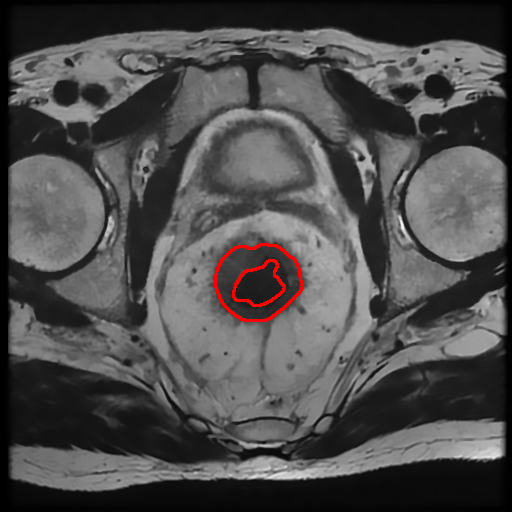
\includegraphics[width=.49\textwidth]{../images/BO56_9_cont.png}
    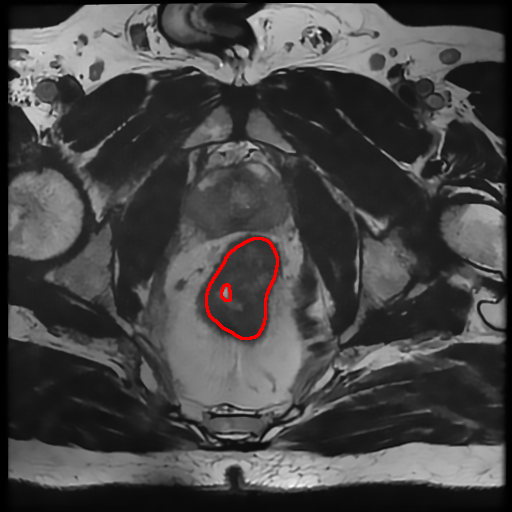
\includegraphics[width=.49\textwidth]{../images/BO85_6_cont.png}
    
    \caption{Images of colorectal cancer with identified tumor areas from two different patients. The red contour represents the border of the predicted tumor area.}
    \label{contoured}
    
    \end{figure}


\end{document}

        % METHODS
        \documentclass{standalone}
\begin{document}
\subsection{Methods}
During the year several segmentation methods have been developed\cite{biondi}.
There are several ways to classify these methods.
For example, depending if they require or not a training set of data, they can be classified into \textit{supervised} or \textit{unsupervised} methods.
More, they can be classified depending on the information type they use, like \textit{Pixel classification} methods, which use only information about pixel intensity, or \textit{Boundary following} methods which use edge information etc...\cite{biondi}.\\
Among the most common ones:

\paragraph{Thresholding}
is a very simple and common approach to segmentation.
This method is applied on the \textit{histogram} of the image.
The histogram of a digital image with intensity levels $L$ in the range $[0, \: L-1]$, is a discrete function $h(l_k) = n_k$ where $l_k$ is the k-th intensity value and $n_k$  is the number of pixels with intensity $l_k$.\\
Thresholding consists in binarizing an image through an (if) clause on the intensity value of each point after having determined a threshold value $T \in [0, \: L-1]$.
The threshold value $T$ is usually chosen by visual assessment on the image histogram but it can be automatize by algorithms like the \textit{Otsu algorithm}.
One drawback of this method is that some parts of the image can belong to the same class even if they belong to different objects.
In fact, thresholding does not take into account the spatial characteristics of the image.
Moreover, it is sensitive to noise and intensity inhomogeneity that corrupt the image histogram and make difficult the classification of pixels\cite{biondi}.

\begin{figure}[htp]

    \centering
    \includegraphics[width=.45\textwidth]{../images/thresholdhistogram.png}
    \includegraphics[width=.45\textwidth]{../images/thresholdexample.png}
    
    \caption{Example of thresholding segmentation using Fiji software\cite{Fiji}. \\
    \textit{ Left)} Image Histogram.\textit{ Right)} Result of thresholding.}
    \label{thresholding}
    
    \end{figure}


\paragraph{Artificial Neural Networks} 
are computational architectures derived from neural physiological models\cite{segmentationreview}.
Artificial Neural Networks (ANNs) have evolved into a broad family of techniques.
For visual analysis are usually used Convolutional Neural Networks (CNNs) based on \textit{convolution kernels} or \textit{filters} that slide along input data to extract feature maps\cite{wiki:cnn}.
Several architectures have been developed over the years, for different tasks and fields of application.
In bio-medical image processing, the so-called U-Net\cite{unet}, is one of the most common architecture.
U-Net is a kind of CNN which allows overcoming the requirement of many training data\cite{biondi, unet}.
However a better explanation of ANNs will be provided in the following chapter.




\end{document}
        
        % UNET
        \documentclass{standalone}
\begin{document}
\section{U-Net}
The U-net is a convolutional network architecture for fast and precise segmentation of images especially in the biomedical field\cite{unet}.
One of the main advantage of the U-net is the ability of dealing with small dataset. The name U-net refers to the U shape of the network architecture. 
The whole structure is divided into two main parts, as shown in Figure\ref{fig:unet}:

\paragraph{Encoder}:
or contraction path is a sequence of convolutional and max pooling layers with the aim of extracting features and reducing dimensionality.

\paragraph{Decoder}:
or expansion path is a sequence of transpose convolutional layers to with the aim of reconstruct the feature map and consequently the segmentation mask.
\begin{figure}[htp]

    \centering
    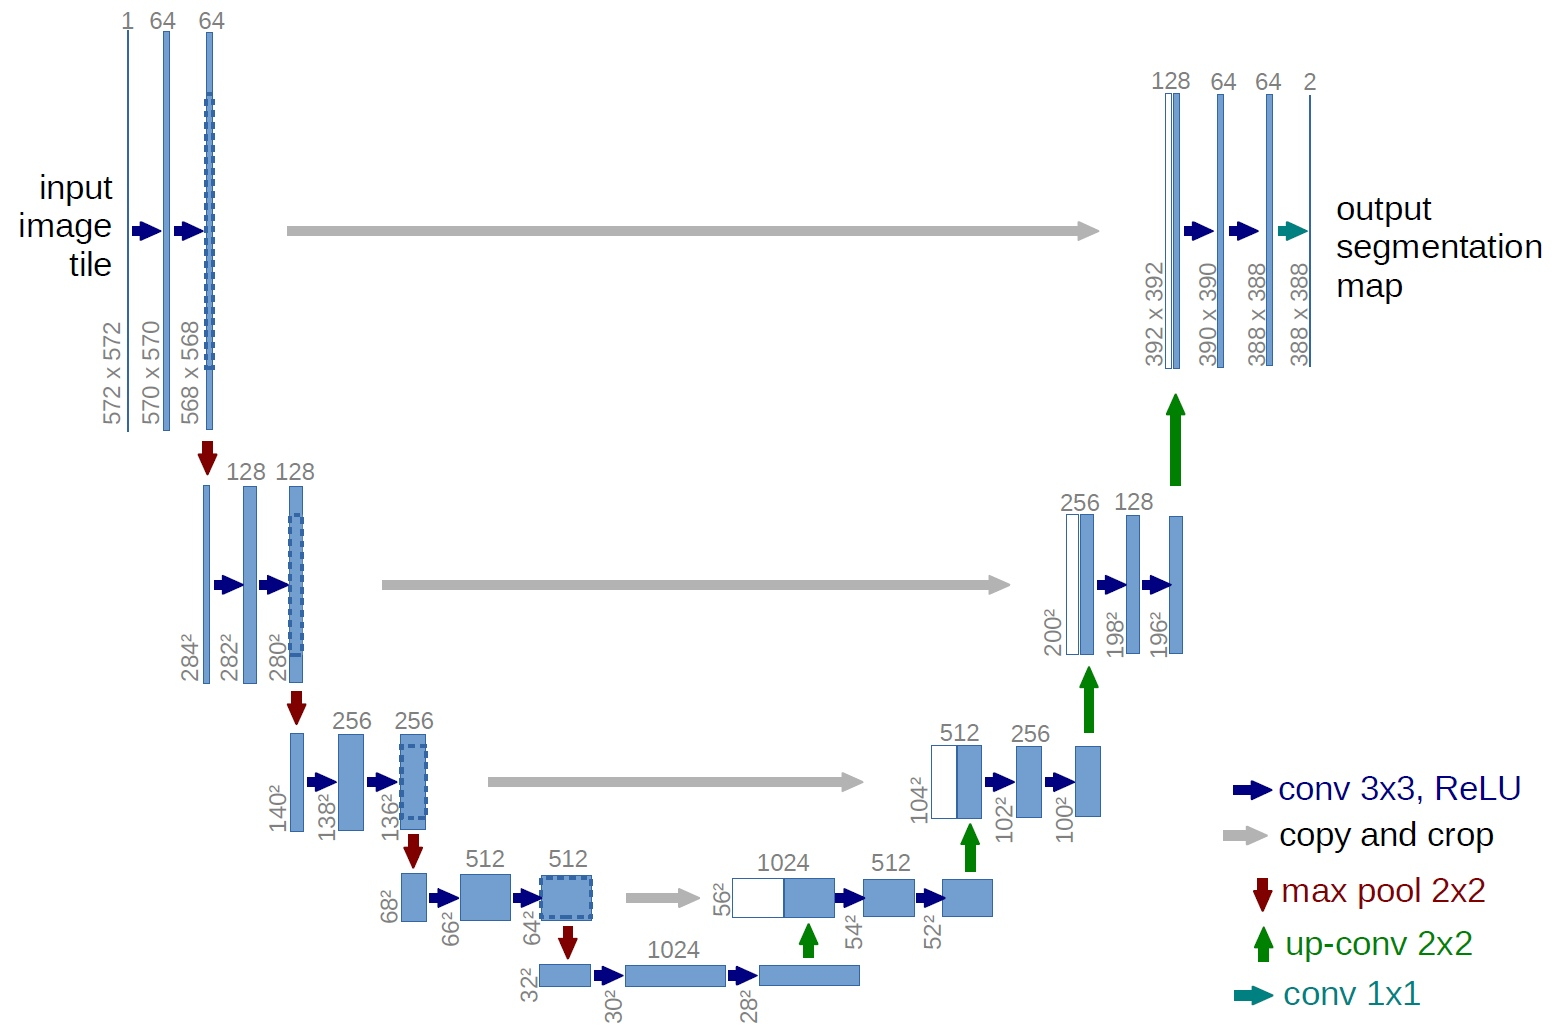
\includegraphics[width=.9\textwidth]{../images/U-Net arch.jpeg}
    
    \caption{Original U-Net architecture. From\cite{unet}}
    \label{fig:unet}
    
    \end{figure}
\\
The \textit{Encoder} is a typical Convolutional Neural Network that consists in the repeated application of convolutions, followed by ReLu activation function and max pooling operations.
During the contraction the input size is decreased and so the spatial information, while the information about features is increased.
The \textit{Decoder} combines the features extracted in the contraction path  with tha spatial information by a sequence of transpose convolutions (or up-convolutions) and concatenations (grey arrows in Figure\ref{fig:unet}).



\end{document}
    
    % RADIOMICS
    \documentclass{standalone}
\begin{document}
\section{Radiomics}
Radiomics consists in methods that extract from medical images a large number of features, which have the potential to uncover disease characteristics that fail to be appreciated by the naked eye\cite{wiki:Radiomics}.
The main objective of radiomics is to assist the subjective interpretation of the clinicians with an objective prediction.
In the new era of precision medicine, radiomics is an emerging translational research field that aims to find associations between qualitative and quantitative information extracted from clinical images and clinical data to support the decision making process\cite{tesicoppola}.
Radiomic features can be divided into different classes:
\begin{itemize}
    \item First Order Statistics
    \item Shape based features 2D and 3D
    \item Gray Level Co-occurrence Matrix (GLCM)
    \item Gray Level Size Zone (GLSZM)
    \item Gray Level Run Length Matrix (GLRLM)
    \item Neighbouring Gray Tone Difference Matrix (NGTDM)
    \item Gray Level Dependence Matrix (GLDM)
\end{itemize}

\end{document}

        % POSSIBLE PURPOSES OF RADIOMICS
        \documentclass{standalone}
\begin{document}
\subsection{Possible Purposes Of Radiomics}

The possible applications of radiomics are based on a very wide range, from the prediction of clinical outcomes to the oncological diagnosis.
In this subsection, a brief overview of some general possible purposes will be given.
\subsubsection{Prediction of clinical outcomes} 
Radiomic features may be useful for predicting patient survival and describing intratumoral heterogeneity as demonstrated in a study by Aerts et al. \cite{Aerts}.
More, the usefulness of radiomics for predicting the immunotherapy response of patients with non-small cell lung cancer (NSCLC) using pretreatment CT and PET-CT images has been demonstrated by other studies\cite{tesicoppola}.
\subsubsection{Prediction of metastases}
Radiomic features can also predict the metastatic stage of tumors. 
For example, many radiomic features were identified as predictors of distant metastasis of lung adenocarcinoma in a study by Coroller et al.\cite{Coroller}.
They concluded that radiomic features may be useful in identifying patients at high risk of developing distant metastases, guiding clinicians in choosing the most effective treatment for individual patients.
\subsubsection{Prediction of physiological events}
Another possible application of radiomics analysis is the prediction of physiological events. 
Indeed, radiomics can be applied for the characterization and investigation of complex physiological events such as brain activity, which is usually studied with specific imaging techniques such as functional magnetic resonance ”fMRI”\cite{tesicoppola}. 


\end{document}
    \newpage
    % PCA
    \documentclass{standalone}
\begin{document}
\markboth{CHAPTER 1. MATERIALS AND METHODS}{1.5. PCA}
\section{Principal Component Analysis}
Principal component analysis (PCA) is a technique to reduce data dimensionality.
It replaces the $n$ original variables by a smaller number, $q$, of linear combinations, called principal components, of the original variables.
The application areas include data compression, image analysis, pattern recognition, regression and classification prediction\cite{PCA}.\\
The most common definition of PCA, due to Hotelling, states that for a set of observed data vectors 
$ \{ \mathbf{t}_{n} \}$, $n \in \{1, \dots, N \} $, the $q$ principal axes $\mathbf{w}_j$, $j \in \{ 1, \dots, q \} $ are those orthonormal axes onto which the retained variance under projection is maximal.
The vectors $\mathbf{w}_j$ are given by the $q$ dominant eigenvectors (i.e. those with the largest associated eigenvalues $\lambda$) of the sample covariance matrix $\mathbf{S} = \sum_{n}^{} ( \mathbf{t_n} - \mathbf{\bar{t}}) ( \mathbf{t_n} - \mathbf{\bar{t}})^T / N$ such that  $ \mathbf{S}\mathbf{w}_j = \lambda_j \mathbf{w_j}$ and where $\mathbf{\bar{t}}$ is the sample mean.
The vector $\mathbf{x}_{n} = \mathbf{W^T} (\mathbf{t_n} - \mathbf{\bar{t}})$, where $ \mathbf{W} = (\mathbf{w}_1 , \mathbf{w}_2 \dots \mathbf{w}_j)$ is thus a q-dimensional reduced representation of the observed vector $\mathbf{t}_{n}$ \cite{PCA}.
As we have mentioned, $\lambda_j$ is just the variance of each new feature dimension.
How to choose an appropriate $q$ depends on the Variance Contribution Rate  $\alpha_j = \lambda_j / \sum_{j}^{} \lambda_j $. 
This can be determined by looking at the cumulative explained variance ratio as a function of the number of components as shown in figure \ref{cumulativevr}.


\begin{figure}[ht]

    \centering
    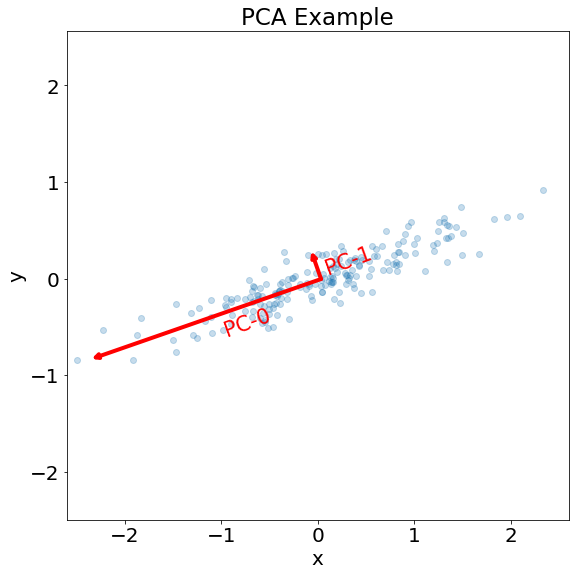
\includegraphics[width=0.62\textwidth]{../images/PCAexample1.png}
    
    \caption{Example of Principal Component Analysis.
     The red vectors represent the principal axes of the data, and the length of the vector is an indication of the variance of the data when projected onto that axis.}
    \label{PCAexample}
    
    \end{figure}

\markboth{CHAPTER 1. MATERIALS AND METHODS}{1.5. PCA}

\begin{figure}[htp]

    \centering
    \includegraphics[width=.68\textwidth]{../images/cumulative3.png}
    
    \caption{Example of cumulative explained variance ratio as a function of the number of components. This curve quantifies how much of the total variance is contained within the first N components. We can see that the first 10 components contain approximately $75 \%$ of the total variance, while to the reach the $100 \%$ you need around 50 components.}
    \label{cumulativevr}
    
    \end{figure}

\end{document}

    % SVM
    \documentclass{standalone}
\begin{document}
\markboth{CHAPTER 1. MATERIALS AND METHODS}{1.6. SVCs}
\section{Support Vector Classifiers}

Support Vector Classifiers (SVCs) are a subclass of Support Vector Machines (SVMs) that are a set of supervised learning methods (i.e. requires training data) used for purposes such as classification and regression.
A Support Vector Machine constructs a hyper-plane or set of hyper-planes in a high or infinite dimensional space.
Intuitively, a good separation is achieved by the hyper-plane that has the largest distance to the nearest training data points of any class (functional margin), since in general the larger the margin the lower the generalization error of the classifier\cite{SVCscikit, Bishop}.\\
For a SVC, mathematically, given training vectors $ \mathbf{x}_i \in \mathbb{R}^p ,  \: i \in \{1,\dots, n\} \:$, in two classes, and a vector $\mathbf{y} \in \{ -1, \: 1 \}^n$ (or $ \{0, \: 1 \}^n$), the goal is to find $\mathbf{w} \in \mathbb{R}^p$ and $b \in \mathbb{R}$ such that the prediction given by $sign(\mathbf{w^T  \mathbf{\Phi(x)}} + b)$ is correct for most samples \cite{SVCscikit}.\\
The function $\Phi(x)$ provides a convenient way of extending the analysis from the input space to a non-linear feature space by using a high-dimensional mapping. 
Finding a linear separating hyperplane in this feature space is equivalent to finding a non linear decision boundary in the input space\cite{SVCmapping}.\\
A SVC solves a primal problem and a dual problem. 
The primal:
\begin{equation}
    \min_{w, \zeta} \frac{1}{2} (\mathbf{w}^T  \mathbf{w}) + C \sum_{i = 1}^{n} \zeta_i
\end{equation}

subject to: $\begin{cases}
    y_i \cdot (\mathbf{w}^T  \mathbf{\Phi(x_i)} + b)  \geq 1 - \zeta_i, \\
    \zeta_i \geq 0 \quad i = 1, \dots, n 
    \end{cases}$
\newline
\\
\\
From an intuitive point of view, the minimization ($\mathbf{w}^T  \mathbf{w}$) corresponds to maximize the functional margin while incurring a penalty when a sample is misclassified or within the margin boundary.
The penalty term C controls the strength of this penalty, and acts as an inverse regularization parameter\cite{SVCscikit}.
Ideally, the term $\zeta_i$ should be 0 for a perfect prediction but real data are usually not always perfectly separable with a hyperplane, so some samples will be at a distance $\zeta_i$ from their correct margin boundary.
\\
The dual problem instead:
\begin{equation}
    \min_{\alpha} \frac{1}{2} (\mathbf{a}^T \mathbf{Q} \mathbf{a}) - \mathbf{e}^T \mathbf{a}
\end{equation}

subject to: $\begin{cases}
    \mathbf{y}^T \mathbf{a} = 0, &  \\
    0 \leq a_i \leq C  &  i = 1, \dots, n
    \end{cases}$
\newline
where $\mathbf{e}$ is the vector of all ones, $\mathbf{Q}$ is a $n \times n$ matrix: $Q_{ij}\equiv y_i y_j K(\mathbf{x_i}, \mathbf{x_j})$ where $K(\mathbf{x_i}, \mathbf{x_j}) = \mathbf{\Phi(x_i)}^T \mathbf{\Phi(x_j)} $ is the so called \textit{kernel}.
The $a_i$ terms are called \textit{dual coefficients}, and they are upper-bounded by C.\\


\newpage
\markboth{CHAPTER 1. MATERIALS AND METHODS}{1.6. SVCs}
Once these problems are solved, for a sample $\mathbf{z}$, the decision function is given by: 
\begin{equation}
    \sum_{i \in SV}^{}  y_i a_i \mathbf{K(x_i, z)} + b
\end{equation}
where the sum is over the supported  vectors (SV) that are the samples that lie within the margin because the dual coefficients $a_i$ are zero for the other samples\cite{SVCscikit}.

\begin{figure}[ht]

    \centering
    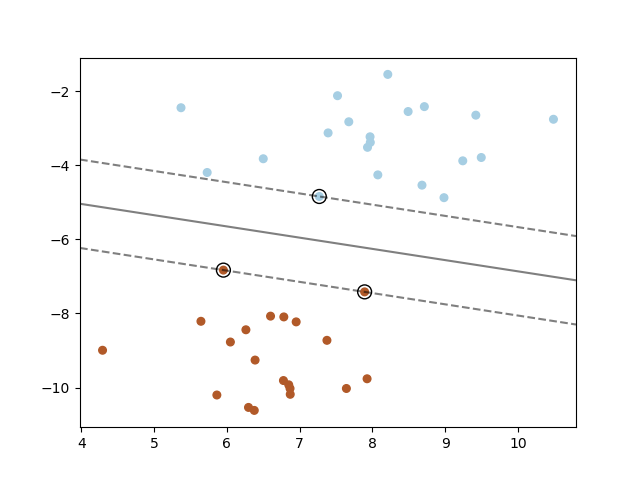
\includegraphics[width=.95\textwidth]{../images/svcexample.png}
    
    \caption{Classification made by a Support Vector Classifier (SVC) for a linearly separable problem. The gray line represents the line of the separation hyper-plane. The three samples on the margin boundaries (dashed lines) are called \textit{support vectors}. From \cite{SVCscikit}}\label{fig:svc}
    
    
    \end{figure}

\end{document}


\end{document}





\documentclass{standalone}
\begin{document}
\chapter*{Conclusions}\addcontentsline{toc}{chapter}{Conclusions}




\end{document}

\clearpage


\printbibliography
%\bibliographystyle{unsrturl}
%\bibliography{bibliography}

\end{document}